\documentclass[11pt]{amsart}
\usepackage[margin=1.15in]{geometry}
\usepackage[T1]{fontenc}
\usepackage{lmodern}
\usepackage{amssymb,amsmath,mathtools}
\usepackage{graphicx,float}
\usepackage[hidelinks]{hyperref}
\usepackage[expansion=false]{microtype}

\newtheorem{theorem}{Theorem}[section]
\newtheorem{proposition}[theorem]{Proposition}
\newtheorem{lemma}[theorem]{Lemma}
\newtheorem{corollary}[theorem]{Corollary}
\newtheorem{mainthm}{Theorem}
\renewcommand{\themainthm}{\Alph{mainthm}}
\theoremstyle{definition}
\newtheorem{definition}[theorem]{Definition}
\newtheorem{remark}[theorem]{Remark}

\newcommand{\RR}{\mathbb{R}}
\newcommand{\Ric}{\mathrm{Ric}}
\newcommand{\FF}{(F\!\cdot\! F)}

\setlength{\emergencystretch}{2.5em}
\hbadness=2000
\raggedbottom
\begin{document}

\title[Kaku's membrane field equations]{The Background Equations of Kaku's\\ Membrane Sigma Model Are Not Integrable}

\author{Deep Bhattacharjee}
\address{Formerly, Electro-Gravitational Space Propulsion Laboratory (EGSPL), Bhubaneswar, Odisha 751030, India}
\address{Formerly, University of Calcutta (Heramba Chandra College), 23/49 Gariahat Road, Golpark, Kolkata 700029, West Bengal, India}
\email{d.bhattacharjee@erl-forschung.de}
\email{itsdeep@live.com}
\email{egspl@proton.me (GitHub-related contact; GitHub account creelie)}
\urladdr{https://orcid.org/0000-0003-0466-750X}

\begin{abstract}
Treating the eleven-dimensional bosonic membrane as a sigma model, Kaku derived the background equations $R_{\mu\nu}+\frac14F_{\mu\alpha\beta\gamma}F_\nu{}^{\alpha\beta\gamma}=0$, $\nabla^\mu F_{\mu\nu\lambda\rho}=0$ at two loops and called the one-loop equations $R_{\mu\nu}=0$, $\nabla^\mu F_{\mu\nu\lambda\rho}=0$ inconsistent. The reverse holds. The one-loop system is integrable, while on every solution of the two-loop system the Bianchi identity forces $F_{\alpha\beta\gamma\delta}F^{\alpha\beta\gamma\delta}$ to be constant, which excludes the membrane solution and the Freund--Rubin vacua. We also show that dimensional regularization, said to be finite in three dimensions, has a pole at $d=3$ at two loops.

\medskip\noindent\textbf{Keywords:} membrane sigma model; eleven-dimensional supergravity; dimensional regularization.

\smallskip\noindent\textbf{MSC 2020:} 83E50 (primary); 81T15, 83E30, 53C25.
\end{abstract}

\maketitle

\section{Introduction}\label{sec:intro}

In string theory the field equations of the background are the conditions under which the two-dimensional sigma model of the string is free of ultraviolet divergences; at one loop they are Einstein's equations coupled to the antisymmetric tensor and the dilaton \cite{CFMP85}. In \cite{Kak00} Kaku set out to repeat this for the membrane. He took the bosonic part of the supermembrane action \cite{BST87} in a background metric $g_{\mu\nu}$ and three-form potential $A_{\mu\nu\lambda}$ on an eleven-dimensional space-time,
\begin{equation}\label{eq:action}
L=\frac{1}{2\alpha}\sqrt{\gamma}\,\gamma^{ij}g_{\mu\nu}\partial_i\phi^\mu\partial_j\phi^\nu+\beta\,\epsilon^{ijk}A_{\mu\nu\lambda}\partial_i\phi^\mu\partial_j\phi^\nu\partial_k\phi^\lambda ,
\end{equation}
expanded it in Riemann normal coordinates by the background field method \cite{AGFM81}, and computed the divergent part of the two-point function of the background. Its vanishing is imposed as the condition on the background, written in terms of $F=dA$, with components $F_{\sigma\mu\nu\lambda}=4\partial_{[\sigma}A_{\mu\nu\lambda]}$.

Two statements of \cite{Kak00} concern us. At one loop the condition reads
\begin{equation}\label{eq:oneloop}
R_{\mu\nu}=0,\qquad \nabla^\mu F_{\mu\nu\lambda\rho}=0,
\end{equation}
and Kaku writes that these equations are ``actually inconsistent'' and that no action of $g$ and $F$ yields them, because a term quadratic in $F$ is missing from the first equation. After a two-loop graph with two insertions of the three-form vertex and a rescaling $\alpha=\alpha_R/\Lambda$ of the coupling by the cut-off, he obtains instead
\begin{equation}\label{eq:twoloop}
R_{\mu\nu}+\tfrac14F_{\mu\alpha\beta\gamma}F_\nu{}^{\alpha\beta\gamma}=0,\qquad \nabla^\mu F_{\mu\nu\lambda\rho}=0,
\end{equation}
which the abstract of the arXiv version of \cite{Kak00} presents as the recovered equations of motion of the background fields. A parenthetical remark in the text notes that no term proportional to $g_{\mu\nu}$ appears and that this signals a ``possible inconsistency'', to be removed for the supermembrane in a later paper; that paper did not appear. The second statement is methodological: dimensional regularization is said to be finite in three dimensions at every loop order, since the momentum integrals only produce Gamma functions of half-integral argument, and point splitting is used instead.

Both statements are false, and the first in a way that removes the main conclusion. Write $\FF_{\mu\nu}=F_{\mu\alpha\beta\gamma}F_\nu{}^{\alpha\beta\gamma}$ and $|F|^2=F_{\alpha\beta\gamma\delta}F^{\alpha\beta\gamma\delta}$.

\begin{mainthm}\label{thm:A}
Let $(M,g)$ be a connected pseudo-Riemannian manifold of dimension eleven and $F$ a closed four-form with $\nabla^\mu F_{\mu\nu\lambda\rho}=0$. If $R_{\mu\nu}=a\FF_{\mu\nu}$ for a constant $a\neq0$, then $|F|^2$ and the scalar curvature are constant on $M$. In particular, the pair \eqref{eq:twoloop} admits no solution with non-constant $|F|^2$, whatever the value of $\beta$.
\end{mainthm}

The constant $a=-\frac14$ in \eqref{eq:twoloop} is fixed by the choice of $\beta$, so Theorem~\ref{thm:A} covers every normalization of the two-loop term. The obstruction disappears only when the trace term of eleven-dimensional supergravity \cite{CJS78} is restored with the right weight.

\begin{mainthm}\label{thm:B}
In the setting of Theorem~\ref{thm:A}, allow $\nabla^\mu F_{\mu\nu\lambda\rho}=\kappa\,(\ast(F\wedge F))_{\nu\lambda\rho}$ for a constant $\kappa$, and consider
\[
R_{\mu\nu}=a\FF_{\mu\nu}+b\,g_{\mu\nu}|F|^2 .
\]
The contracted Bianchi identity is automatic on every solution if and only if $b=-a/12$, which is the ratio in eleven-dimensional supergravity. For every other pair $(a,b)$ with $(a,b)\ne(0,0)$, every solution has constant $|F|^2$. The one-loop system \eqref{eq:oneloop}, the case $a=b=0$, is integrable: every Ricci-flat metric together with every closed and co-closed four-form solves it.
\end{mainthm}

Consequently the Freund--Rubin vacua $\mathrm{AdS}_4\times S^7$ and $\mathrm{AdS}_7\times S^4$ \cite{FR80} and the membrane solution of Duff and Stelle \cite{DS91} solve \eqref{eq:twoloop} for no normalization of the four-form (Corollary~\ref{cor:examples}). The last of these is the field of the membrane itself, and Bergshoeff, Sezgin and Townsend showed that $\kappa$-symmetry of the supermembrane requires the background to satisfy the supergravity equations \cite{BST87}.

\begin{mainthm}\label{thm:C}
For $m>0$ and real $d$ with $2<d<3$ let
\[
S(d)=\int\!\!\int\frac{d^dk}{(2\pi)^d}\frac{d^dl}{(2\pi)^d}\,\frac{1}{(k^2+m^2)(l^2+m^2)((k+l)^2+m^2)}
\]
be the two-loop sunset integral at zero external momentum. Then $S(d)$ is finite and extends to a meromorphic function on $2<\operatorname{Re}d<4$ whose only singularity is a simple pole at $d=3$, with
\[
S(d)=\frac{1}{32\pi^2}\,\frac{1}{3-d}+O(1)\qquad(d\to3).
\]
\end{mainthm}

The sunset is the scalar skeleton of the two-loop graph of \cite{Kak00} formed by two cubic vertices of the expanded action, so the divergence that point splitting was meant to capture is visible in dimensional regularization as an ordinary pole, as in any three-dimensional theory with a two-loop logarithmic divergence \cite{tHV72}.

Section~\ref{sec:identity} proves a divergence identity for closed forms. Section~\ref{sec:bianchi} proves Theorems~\ref{thm:A} and~\ref{thm:B} in any dimension and form degree, Section~\ref{sec:examples} treats the examples and Section~\ref{sec:sunset} proves Theorem~\ref{thm:C}.

\section{A divergence identity}\label{sec:identity}

Throughout, $(M,g)$ is a pseudo-Riemannian manifold of dimension $n$ with Levi-Civita connection $\nabla$, and $F$ is a $p$-form with $p\ge1$. Indices are raised with $g$, and repeated indices are summed over all values, so that for $p=4$
\[
\FF_{\mu\nu}=F_{\mu\alpha_2\cdots\alpha_p}F_\nu{}^{\alpha_2\cdots\alpha_p},\qquad |F|^2=F_{\alpha_1\cdots\alpha_p}F^{\alpha_1\cdots\alpha_p}
\]
agree with the notation of the introduction. We write $J_{\alpha_2\cdots\alpha_p}=\nabla^\mu F_{\mu\alpha_2\cdots\alpha_p}$ for the divergence of $F$.\footnote{With the usual co-differential, $J=-\delta F$; signs play no role below.}

\begin{lemma}\label{lem:div}
If $dF=0$, then
\[
\nabla^\mu\FF_{\mu\nu}=J_{\alpha_2\cdots\alpha_p}F_\nu{}^{\alpha_2\cdots\alpha_p}+\frac{1}{2p}\nabla_\nu|F|^2 .
\]
\end{lemma}

\begin{proof}
By the Leibniz rule $\nabla^\mu\FF_{\mu\nu}=J_{\alpha_2\cdots\alpha_p}F_\nu{}^{\alpha_2\cdots\alpha_p}+T_\nu$ with
\[
T_\nu=F^{\alpha_1\alpha_2\cdots\alpha_p}\nabla_{\alpha_1}F_{\nu\alpha_2\cdots\alpha_p}.
\]
For $1\le k\le p$ let $\widehat{\alpha}_k$ denote the list $\alpha_1,\dots,\alpha_p$ with $\alpha_k$ omitted. Moving $\alpha_k$ to the front of $F^{\alpha_1\cdots\alpha_p}$ costs the sign $(-1)^{k-1}$, so after renaming summation indices
\[
T_\nu=(-1)^{k-1}F^{\alpha_1\cdots\alpha_p}\nabla_{\alpha_k}F_{\nu\widehat{\alpha}_k}\qquad(1\le k\le p),
\]
and averaging over $k$ gives
\begin{equation}\label{eq:Tavg}
T_\nu=\frac1p\,F^{\alpha_1\cdots\alpha_p}\sum_{k=1}^{p}(-1)^{k-1}\nabla_{\alpha_k}F_{\nu\widehat{\alpha}_k}.
\end{equation}
Since $\nabla$ is torsion free, the exterior derivative is the alternation of $\nabla F$:
\[
(dF)_{\nu\alpha_1\cdots\alpha_p}=\nabla_\nu F_{\alpha_1\cdots\alpha_p}+\sum_{k=1}^p(-1)^k\nabla_{\alpha_k}F_{\nu\widehat{\alpha}_k}.
\]
Hence $dF=0$ turns the sum in \eqref{eq:Tavg} into $\nabla_\nu F_{\alpha_1\cdots\alpha_p}$, and $T_\nu=\frac1pF^{\alpha_1\cdots\alpha_p}\nabla_\nu F_{\alpha_1\cdots\alpha_p}=\frac{1}{2p}\nabla_\nu|F|^2$.
\end{proof}

For $p=2$ this is the familiar statement that the Maxwell stress tensor $\FF_{\mu\nu}-\frac14g_{\mu\nu}|F|^2$ is conserved on solutions of the free Maxwell equations; in general it says that $\FF_{\mu\nu}-\frac{1}{2p}g_{\mu\nu}|F|^2$ is conserved when $dF=0$ and $J=0$.

The Chern--Simons current of eleven-dimensional supergravity does not contribute to the first term of Lemma~\ref{lem:div}.

\begin{lemma}\label{lem:cs}
Let $n=11$, $p=4$ and $J=\kappa\ast(F\wedge F)$ for a constant $\kappa$. Then $J_{\alpha\beta\gamma}F_\nu{}^{\alpha\beta\gamma}=0$ for every $\nu$.
\end{lemma}

\begin{proof}
Fix a vector field $X$ and let $\iota_XF$ be the three-form $X^\nu F_{\nu\alpha\beta\gamma}$. Up to a non-zero numerical factor, $X^\nu J_{\alpha\beta\gamma}F_\nu{}^{\alpha\beta\gamma}$ is the pointwise inner product of the three-forms $\iota_XF$ and $\ast(F\wedge F)$, and
\[
\langle\iota_XF,\ast(F\wedge F)\rangle\,\mathrm{vol}=\iota_XF\wedge\ast\ast(F\wedge F)=\pm\,\iota_XF\wedge F\wedge F,
\]
because $\ast\ast=\pm1$ on eight-forms. Contraction is an antiderivation and $F$ has even degree, so $\iota_X(F\wedge F\wedge F)=3\,\iota_XF\wedge F\wedge F$. The left side is the contraction of a twelve-form on an eleven-manifold, hence zero.
\end{proof}

\section{The contracted Bianchi identity}\label{sec:bianchi}

\begin{theorem}\label{thm:general}
Let $(M,g)$ be connected, of dimension $n\ge3$, let $F$ be a closed $p$-form, and suppose
\begin{equation}\label{eq:einsteinform}
R_{\mu\nu}=a\FF_{\mu\nu}+b\,g_{\mu\nu}|F|^2
\end{equation}
with constants $a,b$. Then
\begin{equation}\label{eq:obstruction}
\Big(\frac{a(1-p)}{2p}-\frac{b(n-2)}{2}\Big)\nabla_\nu|F|^2+a\,J_{\alpha_2\cdots\alpha_p}F_\nu{}^{\alpha_2\cdots\alpha_p}=0 .
\end{equation}
\end{theorem}

\begin{proof}
The contracted second Bianchi identity reads $\nabla^\mu R_{\mu\nu}=\frac12\nabla_\nu R$. Taking the trace of \eqref{eq:einsteinform} gives $R=(a+nb)|F|^2$. By Lemma~\ref{lem:div} and $\nabla g=0$,
\[
\nabla^\mu R_{\mu\nu}=a\,J_{\alpha_2\cdots\alpha_p}F_\nu{}^{\alpha_2\cdots\alpha_p}+\Big(\frac{a}{2p}+b\Big)\nabla_\nu|F|^2 .
\]
Subtracting $\frac12(a+nb)\nabla_\nu|F|^2$ gives \eqref{eq:obstruction}.
\end{proof}

\begin{corollary}\label{cor:const}
Under the hypotheses of Theorem~\ref{thm:general}, assume that $J_{\alpha_2\cdots\alpha_p}F_\nu{}^{\alpha_2\cdots\alpha_p}=0$, for instance $J=0$. If
\[
b\ne-\frac{(p-1)\,a}{p\,(n-2)},
\]
then $|F|^2$ and $R$ are constant on $M$. If $b=-(p-1)a/(p(n-2))$, the Bianchi identity imposes no condition.
\end{corollary}

\begin{proof}
The coefficient of $\nabla_\nu|F|^2$ in \eqref{eq:obstruction} vanishes exactly when $b=-(p-1)a/(p(n-2))$. Otherwise $\nabla|F|^2=0$, so $|F|^2$ is constant on the connected manifold $M$, and so is $R=(a+nb)|F|^2$.
\end{proof}

\begin{proof}[Proof of Theorems~\ref{thm:A} and~\ref{thm:B}]
Take $n=11$ and $p=4$. The critical ratio of Corollary~\ref{cor:const} is $b=-3a/36=-a/12$. By Lemma~\ref{lem:cs} the hypothesis $JF=0$ holds when $J=\kappa\ast(F\wedge F)$, including $\kappa=0$. For $b=0$ and $a\ne0$ we are off the critical ratio, which gives Theorem~\ref{thm:A}; the coefficient in \eqref{eq:obstruction} is then $-3a/8$, equal to $3/32$ for Kaku's value $a=-\frac14$. For $(a,b)\neq(0,0)$ off the critical ratio Corollary~\ref{cor:const} gives the constancy of $|F|^2$. When $a=b=0$, equation \eqref{eq:einsteinform} is $R_{\mu\nu}=0$, the Bianchi identity holds identically, and the field equation of $F$ is linear in $F$ for fixed $g$; so any closed and co-closed four-form on any Ricci-flat manifold is a solution, for example a constant four-form on flat $\RR^{1,10}$.

It remains to identify the ratio $b=-a/12$ with supergravity. The bosonic field equations of \cite{CJS78}, for the action $\int\sqrt{|g|}\,(R-\lambda|F|^2)$ plus a Chern--Simons term $\int A\wedge F\wedge F$, read $R_{\mu\nu}-\frac12g_{\mu\nu}R=c\,(\FF_{\mu\nu}-\frac18g_{\mu\nu}|F|^2)$ with $c$ proportional to $\lambda$; the Chern--Simons term does not involve the metric. Taking the trace, $-\frac92R=-\frac38c|F|^2$, so $R=\frac{c}{12}|F|^2$ and
\[
R_{\mu\nu}=c\,\FF_{\mu\nu}-\frac{c}{8}g_{\mu\nu}|F|^2+\frac{c}{24}g_{\mu\nu}|F|^2=c\,\FF_{\mu\nu}-\frac{c}{12}g_{\mu\nu}|F|^2 ,
\]
that is, $b/a=-1/12$.
\end{proof}

\begin{remark}\label{rem:action}
The computation in the last paragraph shows that for every $\lambda\neq0$ the actions $\int\sqrt{|g|}(R-\lambda|F|^2)+\kappa'\int A\wedge F\wedge F$ produce $b/a=-1/12$, so none of them yields \eqref{eq:twoloop}. The pair \eqref{eq:oneloop} is the limit $\lambda\to0$, $\kappa'/\lambda\to0$ of the same family, after the field equation of $A$ is divided by $\lambda$: it describes a test four-form on a Ricci-flat background, a consistent system. What \eqref{eq:oneloop} lacks is the back-reaction of $F$, not consistency, and the attempt to supply the back-reaction through the single term $\FF_{\mu\nu}$ is what produces the obstruction.
\end{remark}

\begin{remark}\label{rem:beta}
In \cite{Kak00} the coefficient of $\FF_{\mu\nu}$ is controlled by $\beta^2\alpha_R^3$, so changing the coupling of the three-form only changes $a$. No choice of couplings produces the trace term $b\,g_{\mu\nu}|F|^2$, and by Corollary~\ref{cor:const} every choice leaves the obstruction $\nabla|F|^2=0$ in place.
\end{remark}

\section{Examples}\label{sec:examples}

\begin{corollary}\label{cor:examples}
For no constant $c\neq0$ is any of the following pairs a solution of \eqref{eq:twoloop}:
\begin{enumerate}
\item the product metric of $\mathrm{AdS}_4\times S^7$ with $F=c\,\mathrm{vol}_{\mathrm{AdS}_4}$;
\item the product metric of $\mathrm{AdS}_7\times S^4$ with $F=c\,\mathrm{vol}_{S^4}$;
\item the membrane of Duff and Stelle \cite{DS91},
\[
ds^2=H^{-2/3}\eta_{ab}\,dx^a dx^b+H^{1/3}\delta_{mn}\,dy^m dy^n,\qquad F=c\,dx^0\wedge dx^1\wedge dx^2\wedge d(H^{-1}),
\]
with $a,b\in\{0,1,2\}$, $m,n\in\{3,\dots,10\}$, $H=1+k/r^6$, $r=|y|$ and $k>0$.
\end{enumerate}
\end{corollary}

\begin{proof}
On a product $M_1\times M_2$ the Ricci tensor is the sum of the Ricci tensors of the factors. In (1), $F$ has no leg along $S^7$, so $\FF_{\mu\nu}=0$ whenever $\mu$ and $\nu$ are tangent to $S^7$, and the first equation of \eqref{eq:twoloop} would force the round seven-sphere to be Ricci flat. In (2) the same argument with the roles of the factors exchanged would force $\mathrm{AdS}_7$ to be Ricci flat. Both are false, since the Ricci tensor of a round sphere or an anti-de Sitter space of radius $\rho$ in dimension $q$ is $\pm(q-1)\rho^{-2}g$.

In (3) the metric is diagonal with $g^{00}=-H^{2/3}$, $g^{11}=g^{22}=H^{2/3}$ and $g^{mm}=H^{-1/3}$, and the only non-zero components of $F$ are $F_{012m}=c\,\partial_m(H^{-1})$ and their permutations. Hence
\[
|F|^2=4!\,g^{00}g^{11}g^{22}\sum_m g^{mm}F_{012m}^2=-24\,c^2H^{5/3}H^{-4}|\nabla H|^2=-864\,c^2k^2\,(r^6+k)^{-7/3},
\]
using $|\nabla H|=6k\,r^{-7}$ and $H^{-7/3}r^{-14}=(r^6+k)^{-7/3}$. This function increases strictly from $-864c^2k^{-1/3}$ at the horizon $r\to0$ to $0$ as $r\to\infty$; see Figure~\ref{fig:m2}. If the pair satisfied \eqref{eq:twoloop}, Theorem~\ref{thm:A} would make $|F|^2$ constant on the connected region $r>0$.
\end{proof}

\begin{figure}[H]
\centering
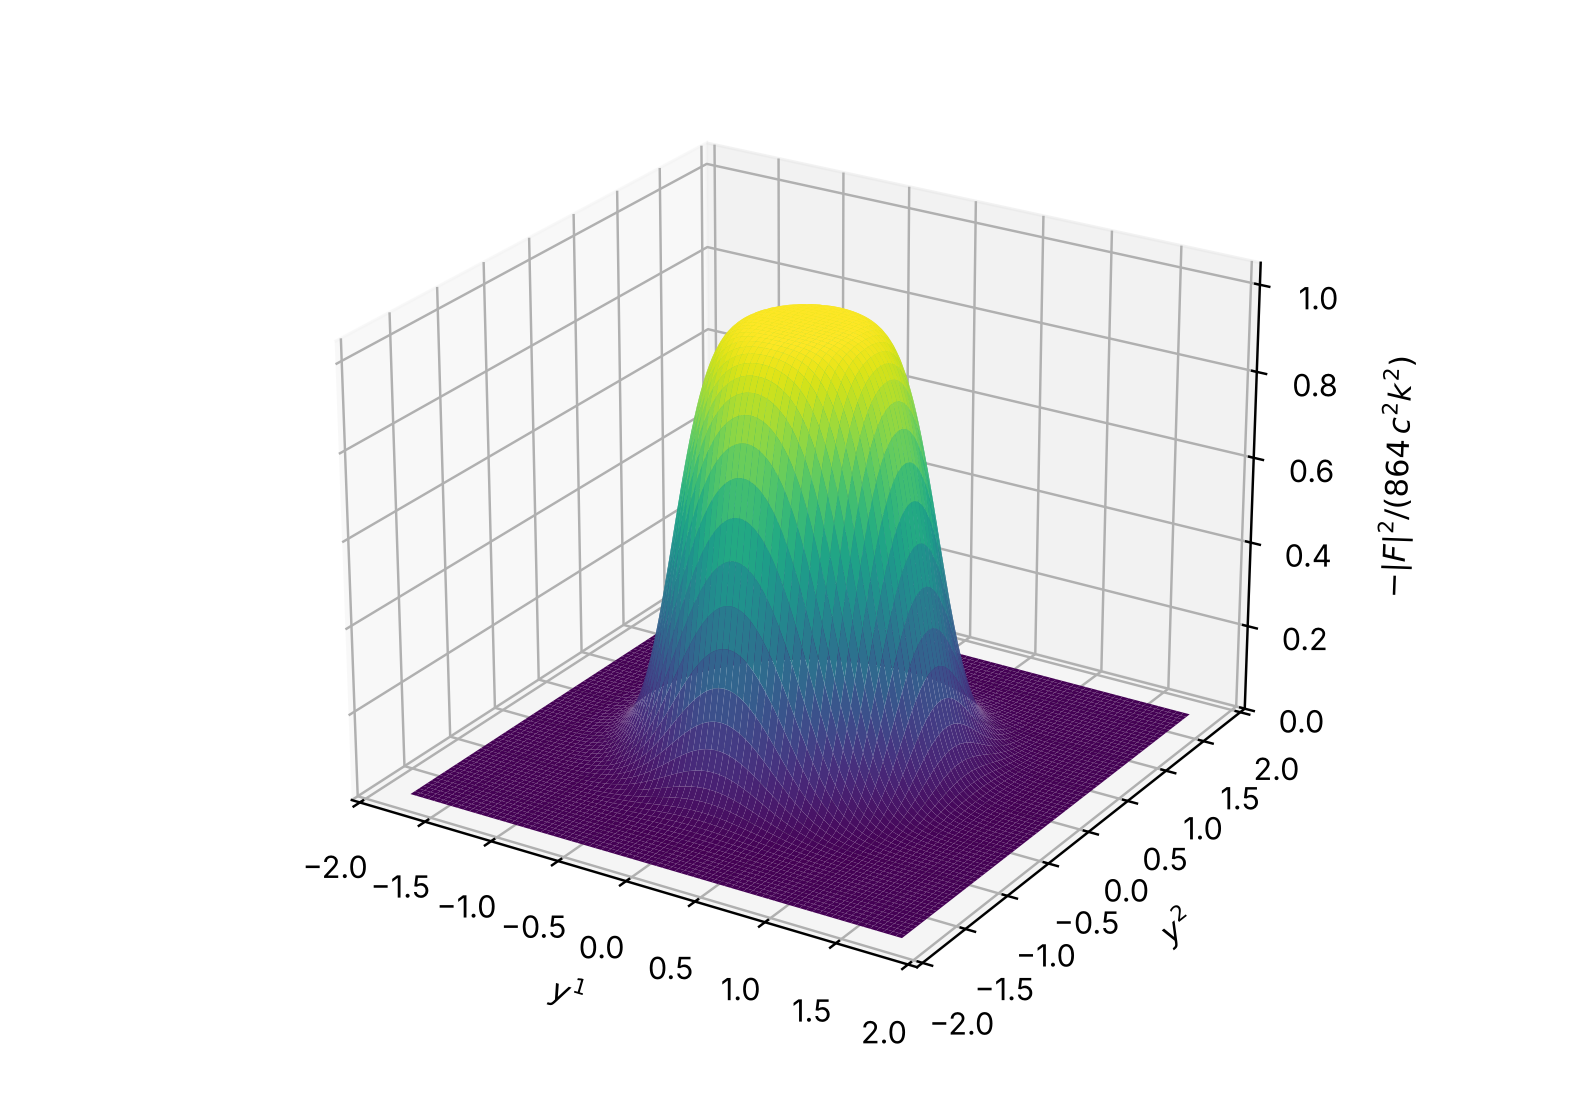
\includegraphics[width=0.82\textwidth]{fig_m2.png}
\caption{The invariant $-|F|^2/(864\,c^2k^2)=(r^6+k)^{-7/3}$ of the Duff--Stelle membrane with $k=1$, over a plane through the membrane in the transverse space. It tends to $k^{-7/3}$ at the horizon, where the geometry approaches $\mathrm{AdS}_4\times S^7$, and to zero at infinity. Theorem~\ref{thm:A} allows only constant profiles.}
\label{fig:m2}
\end{figure}

The first two cases are excluded by \eqref{eq:twoloop} pointwise, without the Bianchi identity; they show that the absence of a trace term already conflicts with the simplest supersymmetric vacua. The third case uses Theorem~\ref{thm:A} and concerns the background created by the membrane whose sigma model is under study. Solutions of \eqref{eq:twoloop} do exist; for example, a product $E\times N$ of a four-dimensional Einstein manifold $E$ with $\Ric_E=6ac^2\epsilon\,g_E$, where $\epsilon=\pm1$ is the sign of $\det g_E$, and a Ricci-flat seven-manifold $N$ solves \eqref{eq:twoloop} with $F=c\,\mathrm{vol}_E$. By Theorem~\ref{thm:A} all solutions share the property that $|F|^2$ is constant.

\section{The two-loop sunset in three dimensions}\label{sec:sunset}

\begin{proof}[Proof of Theorem~\ref{thm:C}]
Let first $d$ be real with $2<d<3$. Write each propagator as $(q^2+m^2)^{-1}=\int_0^\infty e^{-\alpha(q^2+m^2)}\,d\alpha$. The momentum integral is Gaussian:
\[
\int\!\!\int\frac{d^dk\,d^dl}{(2\pi)^{2d}}\,e^{-\alpha_1k^2-\alpha_2l^2-\alpha_3(k+l)^2}=(4\pi)^{-d}\,U^{-d/2},\qquad U=\alpha_1\alpha_2+\alpha_2\alpha_3+\alpha_3\alpha_1,
\]
since $U$ is the determinant of the quadratic form. All integrands are positive, so by Tonelli's theorem
\[
S(d)=(4\pi)^{-d}\int_{(0,\infty)^3}U^{-d/2}e^{-m^2(\alpha_1+\alpha_2+\alpha_3)}\,d\alpha_1\,d\alpha_2\,d\alpha_3 ,
\]
both sides being finite or infinite together. Substitute $\alpha_1=tx$, $\alpha_2=ty$, $\alpha_3=t$ with $x,y,t>0$, of Jacobian $t^2$. Then $U=t^2(xy+x+y)$, and the $t$-integral equals $\Gamma(3-d)\,m^{2d-6}(1+x+y)^{d-3}$. Hence
\begin{equation}\label{eq:sunset}
S(d)=\frac{\Gamma(3-d)\,m^{2d-6}}{(4\pi)^d}\,K(d),\qquad K(d)=\int_0^\infty\!\!\int_0^\infty\frac{(1+x+y)^{d-3}}{(xy+x+y)^{d/2}}\,dx\,dy .
\end{equation}
We show that $K$ is holomorphic on $2<\operatorname{Re}d<4$. Put $s=\operatorname{Re}d$ and $e=\max(s-3,0)$. Since $|(1+x+y)^{d-3}|=(1+x+y)^{s-3}$, on compact subsets of the strip the integrand is dominated by a fixed integrable function, as one checks in three regions. For $x,y\le1$ we have $xy+x+y\ge x+y$ and $1\le1+x+y\le3$, and $(x+y)^{-s/2}$ is integrable near $0\in\RR^2$ because $s<4$. For $x\ge1\ge y$ we have $xy+x+y\ge x$ and $1\le1+x+y\le3x$, so the integrand is at most $3^{e}x^{e-s/2}$, and $e-s/2<-1$ for $2<s<4$; the region $y\ge1\ge x$ is symmetric. For $x,y\ge1$, with $u=\max(x,y)$ and $v=\min(x,y)$, we have $xy+x+y\ge uv$ and $1+x+y\le3u$, so the integrand is at most $3^{e}u^{e-s/2}v^{-s/2}$, and $\int_1^\infty\!\int_1^u u^{e-s/2}v^{-s/2}\,dv\,du<\infty$ for $2<s<4$. In particular $S(d)$ is finite for $2<d<3$, and holomorphy of $K$ follows by dominated convergence. Thus \eqref{eq:sunset} continues $S$ meromorphically to the strip, with poles only where $\Gamma(3-d)$ has them, namely at $d=3$.

At $d=3$ the inner integral is elementary:
\[
\int_0^\infty\frac{dy}{\big((1+x)y+x\big)^{3/2}}=\frac{2}{(1+x)\sqrt{x}},\qquad K(3)=\int_0^\infty\frac{2\,dx}{(1+x)\sqrt x}=2\pi .
\]
Since $\Gamma(3-d)=1/(3-d)+O(1)$, we get $S(d)=(4\pi)^{-3}\,2\pi/(3-d)+O(1)=1/(32\pi^2(3-d))+O(1)$.
\end{proof}

In \cite{Kak00} the absence of poles at $d=3$ is attributed to the Gamma functions of half-integral argument produced by momentum integrations. At two loops the relevant factor is $\Gamma(3-d)$, whose argument is an integer at $d=3$: the superficial degree of divergence of the sunset in three dimensions is $2\cdot3-6=0$, and a logarithmic divergence in any regularization becomes a pole in dimensional regularization. The point-splitting estimates of \cite{Kak00} track only the power divergences.

\section{Discussion}\label{sec:discussion}

The conclusion of \cite{Kak00} that the bosonic membrane sigma model reproduces the background equations at two loops does not survive. The equations \eqref{eq:twoloop} cannot be the field equations of the background: by Theorem~\ref{thm:A} they constrain $|F|^2$ to be constant, which neither follows from an action nor holds for the membrane's own field, and by Theorem~\ref{thm:B} the only Einstein-type equations quadratic in $F$ that avoid the constraint carry the trace term with the supergravity ratio $b/a=-1/12$. The one-loop pair \eqref{eq:oneloop}, which \cite{Kak00} discards as inconsistent, is in fact the integrable system of a test field on a Ricci-flat background. Any derivation of the background equations from the membrane sigma model must therefore produce a counterterm proportional to $g_{\mu\nu}|F|^2$ in the metric sector, as the $\kappa$-symmetry analysis of \cite{BST87} predicts for the supermembrane. Finally, dimensional regularization is available in three dimensions: Theorem~\ref{thm:C} shows that it detects the two-loop logarithmic divergences as poles, so the loss of covariance accepted in \cite{Kak00} for point splitting is not forced.

\section*{Acknowledgements}

The author acknowledges that the membrane sigma model and its expansion studied here are due to Kaku \cite{Kak00}, who based them on the supermembrane of Bergshoeff, Sezgin and Townsend \cite{BST87} and on the covariant background field method of Alvarez-Gaum\'e, Freedman and Mukhi \cite{AGFM81}. The string analogue is the work of Callan, Friedan, Martinec and Perry \cite{CFMP85}. The field equations of eleven-dimensional supergravity are those of Cremmer, Julia and Scherk \cite{CJS78}, the vacua used in Section~\ref{sec:examples} are those of Freund and Rubin \cite{FR80} and of Duff and Stelle \cite{DS91}, and dimensional regularization is that of 't~Hooft and Veltman \cite{tHV72}.

\section*{Declarations}

\noindent\textbf{Data availability.} No data were generated. The \LaTeX\ source and the script that draws the figure are available at \url{https://github.com/creelie/j-4}.

\smallskip\noindent\textbf{Funding.} The author received no funding for this work.

\smallskip\noindent\textbf{Conflict of interest.} The author declares no conflict of interest.

\smallskip\noindent\textbf{Ethics statement.} This work involves no human or animal subjects.

\begin{thebibliography}{99}

\bibitem{AGFM81} L.~Alvarez-Gaum\'e, D.~Z.~Freedman and S.~Mukhi, The background field method and the ultraviolet structure of the supersymmetric nonlinear $\sigma$-model, \emph{Ann. Phys.} \textbf{134} (1981), 85--109. doi:10.1016/0003-4916(81)90006-3.

\bibitem{BST87} E.~Bergshoeff, E.~Sezgin and P.~K.~Townsend, Supermembranes and eleven-dimensional supergravity, \emph{Phys. Lett. B} \textbf{189} (1987), 75--78. doi:10.1016/0370-2693(87)91272-X.

\bibitem{CFMP85} C.~G.~Callan, D.~Friedan, E.~J.~Martinec and M.~J.~Perry, Strings in background fields, \emph{Nucl. Phys. B} \textbf{262} (1985), 593--609. doi:10.1016/0550-3213(85)90506-1.

\bibitem{CJS78} E.~Cremmer, B.~Julia and J.~Scherk, Supergravity theory in eleven dimensions, \emph{Phys. Lett. B} \textbf{76} (1978), 409--412. doi:10.1016/0370-2693(78)90894-8.

\bibitem{DS91} M.~J.~Duff and K.~S.~Stelle, Multi-membrane solutions of $D=11$ supergravity, \emph{Phys. Lett. B} \textbf{253} (1991), 113--118. doi:10.1016/0370-2693(91)91371-2.

\bibitem{FR80} P.~G.~O.~Freund and M.~A.~Rubin, Dynamics of dimensional reduction, \emph{Phys. Lett. B} \textbf{97} (1980), 233--235. doi:10.1016/0370-2693(80)90590-0.

\bibitem{Kak00} M.~Kaku, Ultraviolet behavior of bosonic quantum membranes, \emph{Phys. Rev. D} \textbf{61} (2000), 085025. doi:10.1103/PhysRevD.61.085025. arXiv:hep-th/9907016.

\bibitem{tHV72} G.~'t~Hooft and M.~Veltman, Regularization and renormalization of gauge fields, \emph{Nucl. Phys. B} \textbf{44} (1972), 189--213. doi:10.1016/0550-3213(72)90279-9.

\end{thebibliography}

\end{document}
